\section{Proposed architecture}

\framepic{graphics/architecture/architecture}{
    \framefill
    \textcolor{white}{Proposed architecture}
    \vskip 0.5cm
}

\begin{frame}[fragile]{Proposed architecture}
    \vskip -0.5cm
    \begin{block}{Region-based CNN (R-CNN)}
        \begin{itemize}
            \item Region proposals
            \item Classification
        \end{itemize}
    \end{block}
    \vskip 0.25cm
    \centering
    \begin{tikzpicture}
        % Input
        \node[rectangle, draw, minimum width=2cm, minimum height=2cm, anchor=west] at (-2,0) {Image};

        % \onslide <2-> {
            \draw[->] (0.5,0) -- (1.5,0);

            % Region proposals
            \node at (2.5,1.5) {Region proposals};
            \foreach \i in {0,...,7}
                \node[rectangle, draw, minimum width=1cm, minimum height=1cm, anchor=north west, fill=white] at (2 +\i*0.2,1-\i*0.2) {};
        % }

        % \onslide <3-> {
            \draw[->] (4.5,0) -- (5.5,0);

            % Classification
            \node at (5.5,1.5) {Class};
            \draw[->, color=UniBlue] (6.2, .8) -- (5.7, 1.25);
            \draw[color=UniBlue] (6.35,-.25) ellipse (0.25cm and 1.1cm);

            \node at (8.2,2) {Encoded};
            \node at (8.3,1.5) {Pixels};
            \draw[->, color=UniOrange] (7, .95) -- (7.5, 1.55);
            \draw[color=UniOrange] (7.6,.6) ellipse (1.1cm and 0.35cm);

            \node [matrix, anchor=north west, draw] at (6,1)
            {
                % \node {Class}; & \node {EncodedPixels};\\
                \node {$1$}; & \node {``12 13 \ldots''};\\
                \node {$2$}; & \node {``6 35 \ldots''};\\
                \node {$3$}; & \node {``''};\\
                \node {$4$}; & \node {``192 78 \ldots''};\\
            };
        % }
    \end{tikzpicture}
\end{frame}

\subsection{Region proposals}
\begin{frame}
    \frametitle{Edge-based image segmentation}
    \framesubtitle{Edge Detection}
    \includegraphics[width=\textwidth]{graphics/computervision/edge-odd}
    \includegraphics[width=\textwidth]{graphics/computervision/edge-odd-plot}
    % \begin{exampleblock}{Odd transition}
    %     Given a function defined on a $2D$ domain, a local odd transition is likely to describe border edge.
    % \end{exampleblock}
\end{frame}

% \begin{frame}
%     \frametitle{Edge-based image segmentation}
%     \framesubtitle{Edge Detection}
%     \includegraphics[width=\textwidth]{graphics/computervision/edge-even}
%     \includegraphics[width=\textwidth]{graphics/computervision/edge-even-plot}
%     \begin{exampleblock}{Even transition}
%         Given a function defined on a $2D$ domain, a local even transition is likely to describe a line.
%     \end{exampleblock}
% \end{frame}

\begin{frame}
    \frametitle{Edge-based image segmentation}
    \framesubtitle{Phase Congruency}
    \includegraphics[width=\linewidth]{graphics/architecture/phasecong}
\end{frame}

\begin{frame}
    \frametitle{Edge-based image segmentation}
    \framesubtitle{Kovesi Algorithm}
    \includegraphics[width=\linewidth]{graphics/architecture/gabor}
\end{frame}
    
\begin{frame}
    \frametitle{Edge-based image segmentation}
    \framesubtitle{Kovesi Algorithm}
    \begin{block}{Phase-congruency model}
        Given $z_1, z_2, \ldots, z_n \in \mathcal{V}$, their phase congruency is defined as:
        \begin{equation*}
            \mathcal{P} = \frac{\lvert\sum_{i} z_{i}\rvert}{\sum_{i} \lvert z_{i} \rvert} \in \left[0,1\right],
            % \mathcal{P} (q) = \frac{\max(0,\lvert \sum_{n} z_{n} (q) \rvert - T)}{\sum_{n} r_{n} (q) + \varepsilon} \in \left[0,1\right],
        \end{equation*}
    \end{block}
    \centering
    \includegraphics[width=0.6\textwidth]{graphics/computervision/phasecongruency}
\end{frame}

\begin{frame}
	\frametitle{Edge-based image segmentation}
	\framesubtitle{Kovesi Algorithm}
	\onslide<1-> {
		\includegraphics[width=\textwidth]{graphics/architecture/detector-ex}
	}
	\onslide<2> {
		\includegraphics[width=\textwidth]{graphics/architecture/detector-ex-kovesi}
	}
\end{frame}

\begin{frame}
	\frametitle{Edge-based image segmentation}
	\framesubtitle{Hysteretic Edge Follower}
	\begin{block}{Algorithm}
	  	Let $\mathcal{I}$ be the image, $\mathcal{Q} = \left\{q \in \mathcal{I} \colon \hat{\mathcal{P}}(q) > T_{high}\right\}$, $\Omega(q)$ the set of  pixels adjacent to $q$ and $\mathcal{E} = \empty$ the set of edge pixels.
		Then, the hysteretic edge follower calculates edge pixels as:
		\begin{enumerate}
			\item $q_i \in \mathcal{Q};\; \mathcal{Q} = \mathcal{Q} \setminus \{q_i\};\;\mathcal{E} = \mathcal{E} \cup \{q_i\}$
			\item $\forall q_j \in \Omega(q_i)$ if $\hat{\mathcal{P}}(q_j) > T_{low}$ then $\mathcal{E} = \mathcal{E} \cup \{q_j\}$ and repeat $(2)$ with $q_i = q_j$
			\item if $\mathcal{Q} \neq \emptyset$ then repeat $(1)$
		\end{enumerate}
	\end{block}
\end{frame}

\begin{frame}
	\frametitle{Edge-based image segmentation}
	\framesubtitle{Hysteretic Edge Follower}
	\only<1-4> {
		\includegraphics[width=\textwidth]{graphics/architecture/detector-ex}
	}
	\only<2-4> {
		\includegraphics[width=\textwidth]{graphics/architecture/detector-ex-hysteresis-30-50}
	}
	\only<3-4> {
		\includegraphics[width=\textwidth]{graphics/architecture/detector-ex-hysteresis-60-100}
	}
	\only<4-4> {
		\includegraphics[width=\textwidth]{graphics/architecture/detector-ex-hysteresis-90-150}
	}
\end{frame}

\begin{frame}
    \frametitle{Edge-based image segmentation}
    \framesubtitle{$\alpha$-Shape}
    \begin{columns}[onlytextwidth]
        \column{0.5\textwidth}
            \onslide <1-> {
                \includegraphics[width=\textwidth]{graphics/computervision/detector-points}
            }
        \column{0.5\textwidth}
            \onslide <2-> {
                \includegraphics[width=\textwidth]{graphics/computervision/detector-a-shape-better-radius}
            }
    \end{columns}
%    \onslide <3-> {
%        \begin{theorem}[Topologically correct image segmentation]
%            Under certain conditions on the parameters of the alpha-shape, the boundary reconstruction is topologically equivalent to the boundary of the original region.
%        \end{theorem}
%    }
\end{frame}

\begin{frame}
	\frametitle{Edge-based image segmentation}
	\framesubtitle{$\alpha$-Shape}
	\only<1-3> {
			\includegraphics[width=\textwidth]{graphics/architecture/detector-ex}
	}
	\only<2-3> {
			\includegraphics[width=\textwidth]{graphics/architecture/detector-ex-segmentated}
	}
	\only<3-3> {
			\includegraphics[width=\textwidth]{graphics/architecture/detector-ex-bounding-box}
	}
\end{frame}

% \begin{frame}
%     \frametitle{Region proposals}
%     \framesubtitle{Optimization}
%     \onslide <1-> {
%         \begin{alertblock}{Kovesi algorithm tuning}
%             Parameters: $N$, $U$, $\lambda$ and $s$.
%         \end{alertblock}
%     }
%     \onslide <2-> {
%         \begin{alertblock}{Hysteretic edge follower tuning}
%         	Parameters: $T_{low}$ and $T_{high}$.
%         \end{alertblock}
%     }
%     \onslide <3-> {
%         \begin{alertblock}{Alpha shape tuning}
%         	Parameters: $\alpha$, $T_{hole}$ and $T_{regions}$.
%         \end{alertblock}
%     }
%     \onslide <3-> {
%         \begin{exampleblock}{Parameters tuning - solution}
%             An empirical approach is proposed: \textbf{Bayesian optimization} is used to tune the hyper parameters of the algorithm.
%         \end{exampleblock}
%     }
% \end{frame}

\begin{frame}
	\frametitle{Region proposals}
    \framesubtitle{Optimization}
    \onslide<1-> {
        \begin{block}{Accuracy}
            \begin{equation*}
            \mathcal{A} = \frac{\lvert X \cap Y \rvert}{\lvert Y \rvert}
            \end{equation*}
        \end{block}
    }
	\onslide<2-> {
        \begin{block}{Loss function}
            \begin{equation*}
            \mathcal{L} = 1 - 2 \frac{\lvert X \cap Y \rvert}{\lvert X \rvert + \lvert Y \rvert}
            \end{equation*}
        \end{block}
    }
    \onslide<3-> {
        \begin{itemize}
            \item Bayesian Optimization
        \end{itemize}
    }
\end{frame}

% \begin{frame}
%     \frametitle{Region proposals}
%     \framesubtitle{Results}
%     \vskip -0.5cm
% 	\begin{table}
% 		\centering
% 		\small	
% 		\begin{tabular}{|c|c|c|c|c|c|}
% 			\hline		
% 			\textbf{No.} & \textbf{Equal.} & \textbf{MinMax} & \textbf{Batch} & \textbf{Loss} & \textbf{Accuracy}\\ \hline
% 			\multirow{3}{*}{1} & no & no & 1024 & 0.8773 & 0.6234 \\
% 			& no & yes & 1024 & \textbf{0.8378} & \textbf{0.5477} \\
% 			& yes & no & 1024 & 0.9205 & 0.6752 \\
% 			& yes & yes & 1024 & 0.7977 & 0.4925 \\ \hline
% 			\multirow{3}{*}{2} & no & no & 760 & 0.9103 & 0.7318\\
% 			& no & yes & 760 & \textbf{0.9061} & \textbf{0.7738} \\
% 			& yes & no & 760 & 0.9676 & 0.9587 \\
% 			& yes & yes & 760 & 0.9172 & 0.3333 \\ \hline
% 			\multirow{3}{*}{3} & no & no & 1024 & 0.7382 & 0.6710 \\
% 			& no & yes & 1024 & \textbf{0.6852} & \textbf{0.6168} \\
% 			& yes & no & 1024 & 0.8161 & 0.9145 \\
% 			& yes & yes & 1024 & 0.6995 & 0.4600 \\ \hline
% 			\multirow{3}{*}{4} & no & no & 1024 & 0.6261 & 0.6190 \\
% 			& no & yes & 1024 & \textbf{0.6455} & \textbf{0.7528} \\
% 			& yes & no & 1024 & 0.6694 & 0.7334 \\
% 			& yes & yes & 1024 & 0.6050 & 0.5550 \\ \hline
% 		\end{tabular}
% 	\end{table}
% \end{frame}

\begin{frame}
	\frametitle{Region proposals}
	\framesubtitle{Example: Class No.1}
    \only<1-4> {
		\includegraphics[width=\textwidth]{graphics/results/detector-result-class1-1}
	}
	\only<2-4> {
		\includegraphics[width=\textwidth]{graphics/results/detector-result-class1-2}
	}
	\only<3-4> {
		\includegraphics[width=\textwidth]{graphics/results/detector-result-class1-3}
	}
	\only<4> {
		\includegraphics[width=\textwidth]{graphics/results/detector-result-class1-4}
	}
\end{frame}

\begin{frame}
\frametitle{Region proposals}
\framesubtitle{Example: Class No.2}
	\only<1-4> {
		\includegraphics[width=\textwidth]{graphics/results/detector-result-class2-1}
	}
	\only<2-4> {
		\includegraphics[width=\textwidth]{graphics/results/detector-result-class2-2}
	}
	\only<3-4> {
		\includegraphics[width=\textwidth]{graphics/results/detector-result-class2-3}
	}
	\only<4> {
		\includegraphics[width=\textwidth]{graphics/results/detector-result-class2-4}
	}
\end{frame}

\begin{frame}
\frametitle{Region proposals}
\framesubtitle{Example: Class No.3}
	\only<1-4> {
		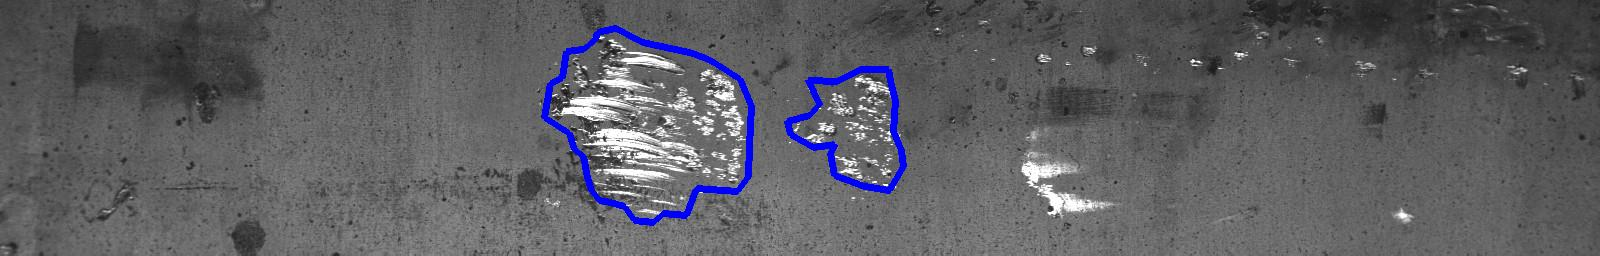
\includegraphics[width=\textwidth]{graphics/results/detector-result-class3-1}
	}
	\only<2-4> {
		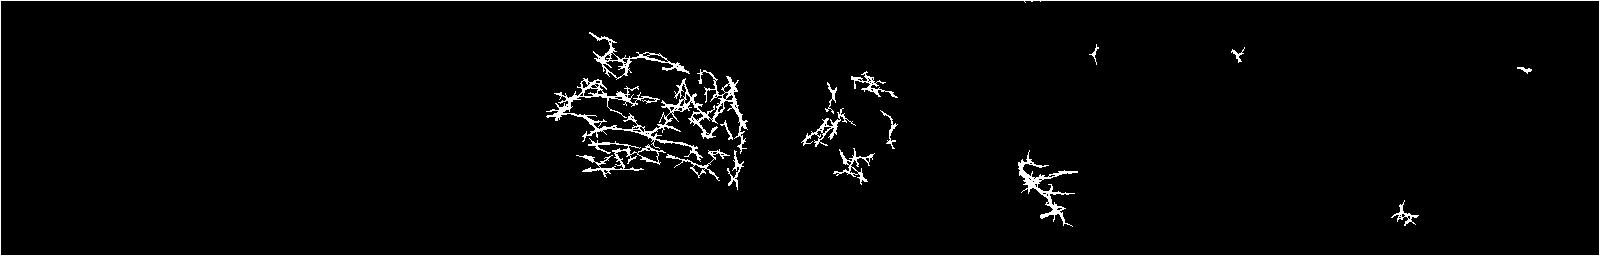
\includegraphics[width=\textwidth]{graphics/results/detector-result-class3-2}
	}
	\only<3-4> {
		
\includegraphics[width=\textwidth]{graphics/results/detector-result-class3-3}
	}
	\only<4> {
		
\includegraphics[width=\textwidth]{graphics/results/detector-result-class3-4}
	}
\end{frame}

\begin{frame}
\frametitle{Region proposals}
\framesubtitle{Example: Class No.4}
	\only<1-4> {
		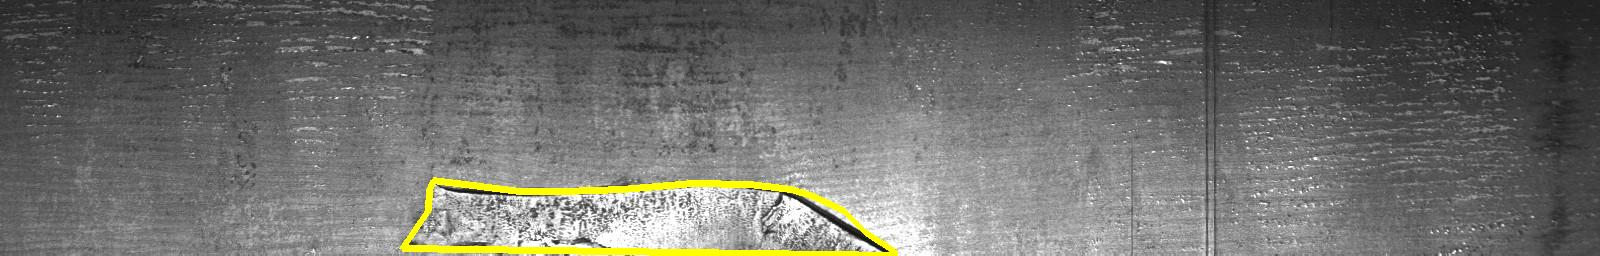
\includegraphics[width=\textwidth]{graphics/results/detector-result-class4-1}
	}
	\only<2-4> {
		
\includegraphics[width=\textwidth]{graphics/results/detector-result-class4-2}
	}
	\only<3-4> {
		
\includegraphics[width=\textwidth]{graphics/results/detector-result-class4-3}
	}
	\only<4> {
		
\includegraphics[width=\textwidth]{graphics/results/detector-result-class4-4}
	}
\end{frame}

\subsection{MC-CNN}
\begin{frame}{Multi Column CNN (MC-CNN)}
    \centering
    \begin{tikzpicture}
        % image
        \node[circle, draw] (input) at (0,0) {I};

        % preprocessed image
        \node[rectangle, draw] (p1) at ($(input) + (2,2)$) {P};
        \node[rectangle, draw] (p2) at ($(input) + (2,.5)$) {P};
        \node (p3) at ($(input) + (2,-.5)$) {\vdots};
        \node[rectangle, draw] (p4) at ($(input) + (2,-2)$) {P};

        % image to preprocessed image
        \draw[->] ($(input) + (0.5, 0)$) -- ($(p1) + (-0.3, 0)$);
        \draw[->] ($(input) + (0.5, 0)$) -- ($(p2) + (-0.3, 0)$);
        \draw[->] ($(input) + (0.5, 0)$) -- ($(p4) + (-0.3, 0)$);

        % cnn
        \node[rounded rectangle, draw, minimum width=2.5cm, minimum height=1cm] (cnn1) at ($(p1) + (2.5,0)$) {CNN};
        \node[rounded rectangle, draw, minimum width=2.5cm, minimum height=1cm] (cnn2) at ($(p2) + (2.5,0)$) {CNN};
        \node[minimum width=2.5cm, minimum height=1cm] (cnn3) at ($(p3) + (2.5,0)$) {\vdots};
        \node[rounded rectangle, draw, minimum width=2.5cm, minimum height=1cm] (cnn4) at ($(p4) + (2.5,0)$) {CNN};

        % preprocessed to cnn
        \draw[->] ($(p1) + (0.5, 0)$) -- ($(cnn1) + (-1.2, 0)$);
        \draw[->] ($(p2) + (0.5, 0)$) -- ($(cnn2) + (-1.2, 0)$);
        \draw[->] ($(p4) + (0.5, 0)$) -- ($(cnn4) + (-1.2, 0)$);

        % classifier
        \node[rectangle, draw, minimum width=2cm, minimum height=1cm] (classifier) at ($(cnn3) + (3.5,0.5)$) {NN};

        % cnn to classifier
        \draw[->] ($(cnn1) + (1.3, 0)$) -- ($(classifier) + (-1.2, .2)$);
        \draw[->] ($(cnn2) + (1.3, 0)$) -- ($(classifier) + (-1.2, 0)$);
        \draw[->] ($(cnn4) + (1.3, 0)$) -- ($(classifier) + (-1.2, -.2)$);

        % output
        \node[circle, draw] (output) at ($(classifier) + (2,0)$) {O};

        % classifier to output
        \draw[->] ($(classifier) + (1.1, 0)$) -- ($(output) + (-.45, 0)$);

    \end{tikzpicture}
\end{frame}

\begin{frame}{Multi Column CNN (MC-CNN)}
    \includegraphics[width=\textwidth]{graphics/architecture/mc-cnn-input}
    $$\Downarrow$$
    \centering
    \begin{tabular}{|c|c|c|c|c|}
        \hline
        Flawless area & Defect \#1 & Defect \#2 & Defect \#3 & Defect \#4\\\hline
        $1\%$ & $4\%$ & $6\%$ & \cellcolor{UniBlue}\textcolor{white}{$87\%$} & $2\%$ \\
        \hline
    \end{tabular}
\end{frame}

% \subsection{Output layer}
\begin{frame}{Output layer}
    \begin{tikzpicture}

        % columns
        \node[rounded rectangle, draw, minimum width = 2cm, minimum height=1cm] (cnn1) at (0,2) {Shape};
        \node[rounded rectangle, draw, minimum width = 2cm, minimum height=1cm] (cnn2) at (0,0) {Local};
        \node[rounded rectangle, draw, minimum width = 2cm, minimum height=1cm] (cnn3) at (0,-2) {Global};

        % columns output
        \foreach \i in {0,...,4}
            \node[rectangle, draw, minimum width=1cm, minimum height=1cm, anchor=north west, fill=white] (output1 \i) at ($(cnn1) + (2+\i*0.15, 1-\i*.15) $) {$87\%$};

        \foreach \i in {0,...,4}
            \node[rectangle, draw, minimum width=1cm, minimum height=1cm, anchor=north west, fill=white] (output2 \i) at ($(cnn2) + (2+\i*0.15, 1-\i*.15) $) {$92\%$};

        \foreach \i in {0,...,4}
            \node[rectangle, draw, minimum width=1cm, minimum height=1cm, anchor=north west, fill=white] (output3 \i) at ($(cnn3) + (2+\i*0.15, 1-\i*.15) $) {$42\%$};

        % columns to output
        \draw[->] ($(cnn1) + (1, 0)$) -- ($(cnn1) + (1.7, 0)$);
        \draw[->] ($(cnn2) + (1, 0)$) -- ($(cnn2) + (1.7, 0)$);
        \draw[->] ($(cnn3) + (1, 0)$) -- ($(cnn3) + (1.7, 0)$);

        % fuse output
        \node [matrix, anchor=west, draw] (finalinput) at ($(cnn2) + (4.5,0)$)
        {
            \node {$13\%$};\\
            \node {$25\%$};\\
            \node {\vdots};\\
            \node {$42\%$};\\
        };

        % cnn output to flatten
        \draw[->] ($(output1 4) + (.6, 0)$) -- ($(finalinput) + (-.7,.2)$);
        \draw[->] ($(output2 4) + (.6, 0)$) -- ($(finalinput) + (-.7,0)$);
        \draw[->] ($(output3 4) + (.6, 0)$) -- ($(finalinput) + (-.7,-.2)$);

        % hidden layer
        \foreach \i in {0,...,7}
            \node[circle, draw, minimum width=.75cm, minimum height=.75cm, anchor=west] (h \i) at ($(finalinput) + (2, 3-\i*.8) $) {};
        \foreach \i in {0,...,7}
            \draw ($(finalinput) + (.75,0)$) -- ($(h \i) + (-.5,0)$);

        % output layer
        \foreach \i in {0,...,4}
            \node[circle, draw, minimum width=.75cm, minimum height=.75cm, anchor=west] (o \i) at ($(finalinput) + (4, 1.75-\i*.8) $) {};
        \foreach \i in {0,...,4}
            \foreach \j in {0,...,7}
                \draw ($(h \j) + (.5,0)$) -- ($(o \i) + (-.5,0)$);
        
        
    \end{tikzpicture}
\end{frame}

% \begin{frame}
%     \frametitle{Multi Column CNN (MC-CNN)}
%     \framesubtitle{Shape column}
%     \includegraphics[width=\textwidth]{graphics/architecture/mc-cnn-shape}
%     % \includegraphics[width=\textwidth]{graphics/architecture/mc-cnn-shape-architecture}
%     TODO confusion matrix + learning curve
% \end{frame}

% \begin{frame}
%     \frametitle{Multi Column CNN (MC-CNN)}
%     \framesubtitle{Local column}
%     \includegraphics[width=\textwidth]{graphics/architecture/mc-cnn-local}
%     % \includegraphics[width=\textwidth]{graphics/architecture/mc-cnn-shape-architecture}
%     TODO confusion matrix + learning curve
% \end{frame}

% \begin{frame}
%     \frametitle{Multi Column CNN (MC-CNN)}
%     \framesubtitle{Global column}
%     \includegraphics[width=\textwidth]{graphics/architecture/mc-cnn-global}
%     % \includegraphics[width=\textwidth]{graphics/architecture/mc-cnn-shape-architecture}
%     TODO confusion matrix + learning curve
% \end{frame}

\begin{frame}
    \frametitle{Convolutional Neural Network (CNN)}
    \begin{columns}
        \column{.5\textwidth}
        \onslide<1-> {\includegraphics[width=\linewidth]{graphics/architecture/convolutionlayer}}
        \column{.5\textwidth}
        \onslide<2-> {\includegraphics[width=\linewidth]{graphics/architecture/poolinglayer}}
    \end{columns}

\end{frame}

\begin{frame}
    \frametitle{Multi Column CNN (MC-CNN)}
    \framesubtitle{Local column}
    \begin{columns}
        \column{.4\textwidth}
            \centering
            \only<1> {\localcolumnnospreader{ForestGreen}{black}{black}{black}{black}{black}}
            % \only<6-7> {\localcolumn{black}{ForestGreen}{black}{black}{black}{black}}
            \only<2-3> {\localcolumnnospreader{black}{black}{ForestGreen}{black}{black}{black}}
            \only<4-5> {\localcolumnnospreader{black}{black}{black}{ForestGreen}{black}{black}}
            \only<6> {\localcolumnnospreader{black}{black}{black}{black}{ForestGreen}{black}}
            \only<7> {\localcolumnnospreader{black}{black}{black}{black}{black}{ForestGreen}}
            \only<8-> {\localcolumn{black}{UniOrange}{black}{black}{black}{black}}
        \column{.6\textwidth}
            \only<1> {
                \begin{itemize}
                    \item \textbf{Input Layer}
                    \item $\left[256\times 1600\times 1\right]$ image
                    \item ``zerocenter'' normalization
                    % \item Activations: $256\times 1600 \times 1 = 409.600$
                \end{itemize}
            }
            \only<8> {
                \begin{itemize}
                    \item \textbf{Spreader Layer}
                    \item $4$ $\left[3\times 3\times 1\right]$ filters
                    \item Stride $\left[1\;1\right]$
                    \item Dilation Factor $\left[400\;400\right]$
                    \item Padding $\left[672\;0\right]$
                    % \item Activations: $800\times 800\times 4 = 2.560.000$
                    % \item Learnables: $3\times 3\times 1 \times 4 = 36$ (Weights) + $1\times 1\times 4 = 4$ (Bias) $ = 40$
                \end{itemize}
            }
            \only<9> {
                \includegraphics[width=\linewidth]{graphics/architecture/dilation2x2}
                \includegraphics[width=\linewidth]{graphics/architecture/dilation3x3}
                \begin{tikzpicture}
                    \node[circle, draw] (downsampling) at (0,0) {$\downarrow$};
                    \draw[->] ($(downsampling) + (-2,0)$) -- node[above] {$\mathcal{I}\left(x,y\right)$} ($(downsampling) + (-.5,0)$);
                    \node[rectangle, draw,minimum height=.75cm,minimum width=1.5cm] (filter) at ($(downsampling) + (2,0)$) {g};
                    \draw[->] ($(downsampling) + (.5,0)$) -- ($(filter) + (-1,0)$);
                    \draw[->] ($(filter) + (1,0)$) -- node[above] {$\mathcal{A}\left(x,y\right)$} ($(filter) + (2.5,0)$);
                \end{tikzpicture}
            }
            \only<10> {
                \spreader{0}{0}{$\mathcal{A}\left(0,0\right) = f_9 \times \mathcal{I}_9 + b$}
            }
            \only<11> {
                \spreader{.175}{0}{$\mathcal{A}\left(400,0\right) = f_8 \times \mathcal{I}_8 + b$}
            }
            \only<12> {
                \spreader{.35}{0}{$\mathcal{A}\left(800,0\right) = f_7 \times \mathcal{I}_7 + b$}
            }
            \only<13> {
                \spreader{0}{-.175}{$\mathcal{A}\left(0,400\right) = f_6 \times \mathcal{I}_6 + b$}
            }
            \only<14> {
                \spreader{.175}{-.175}{$\mathcal{A}\left(400,400\right) = f_5 \times \mathcal{I}_5 + b$}
            }
            \only<15> {
                \spreader{.35}{-.175}{$\mathcal{A}\left(800,400\right) = f_4 \times \mathcal{I}_4 + b$}
            }
            \only<16> {
                \spreader{0}{-.35}{$\mathcal{A}\left(0,800\right) = f_3 \times \mathcal{I}_3 + b$}
            }
            \only<17> {
                \spreader{.175}{-.35}{$\mathcal{A}\left(400,800\right) = f_2 \times \mathcal{I}_2 + b$}
            }
            \only<18> {
                \spreader{.35}{-.35}{$\mathcal{A}\left(800,800\right) = f_1 \times \mathcal{I}_1 + b$}
            }
            \only<19> {
                \centering
                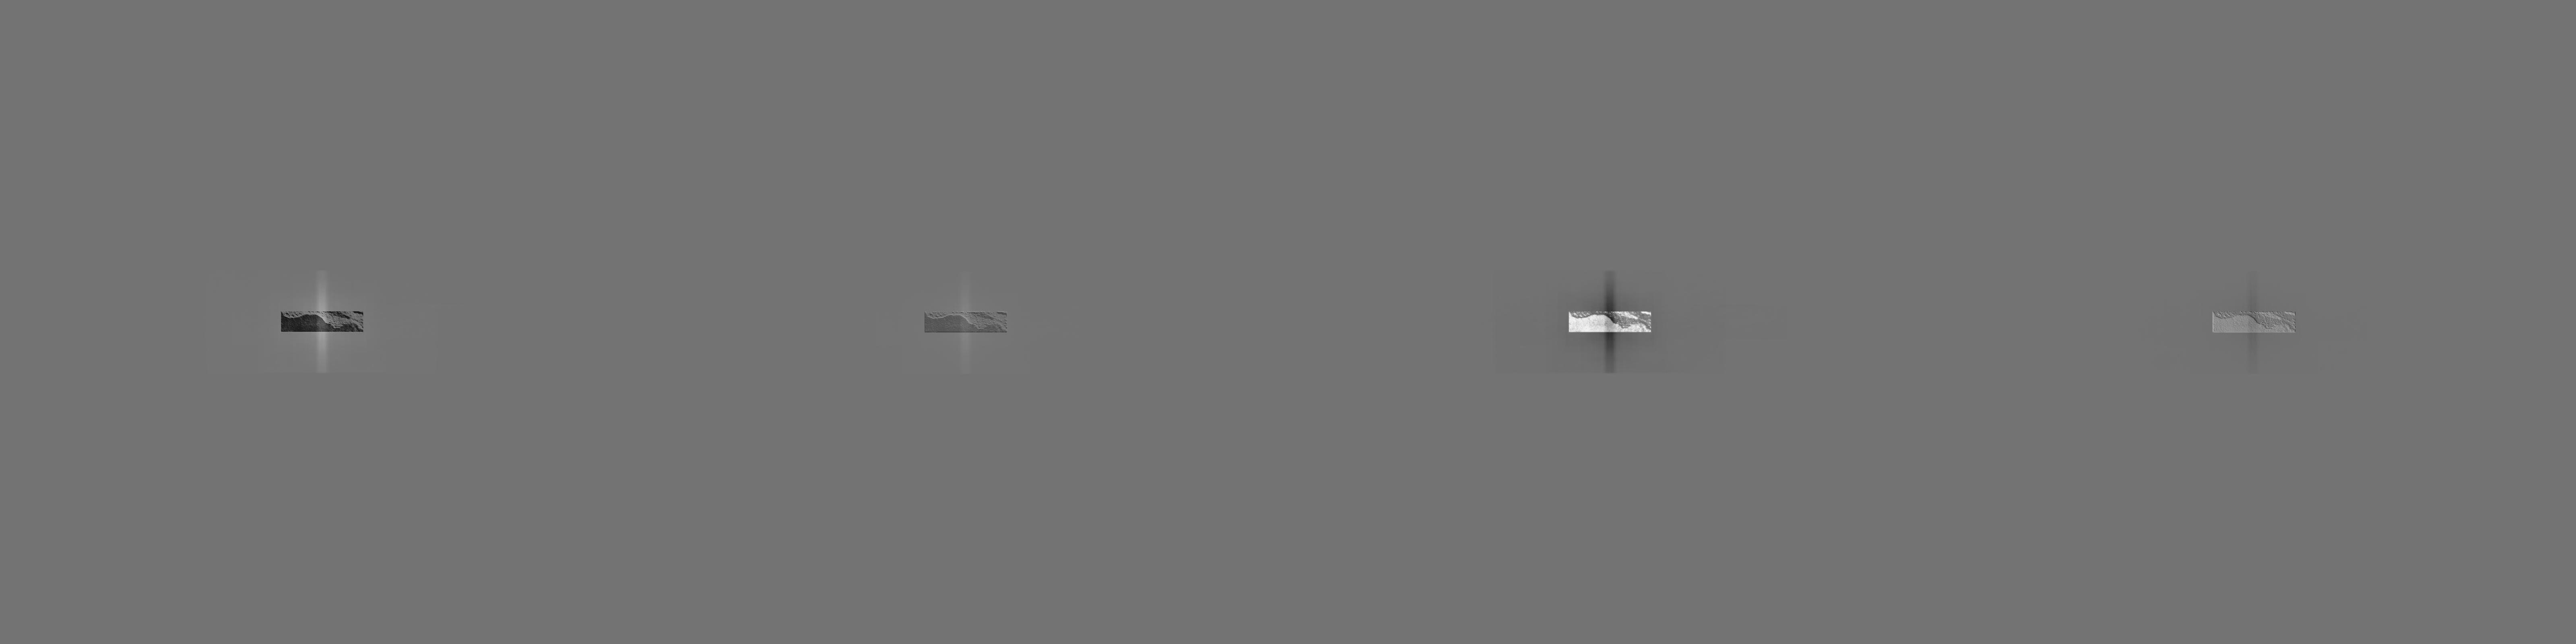
\includegraphics[width=\textwidth,angle=90]{graphics/architecture/act_net}
                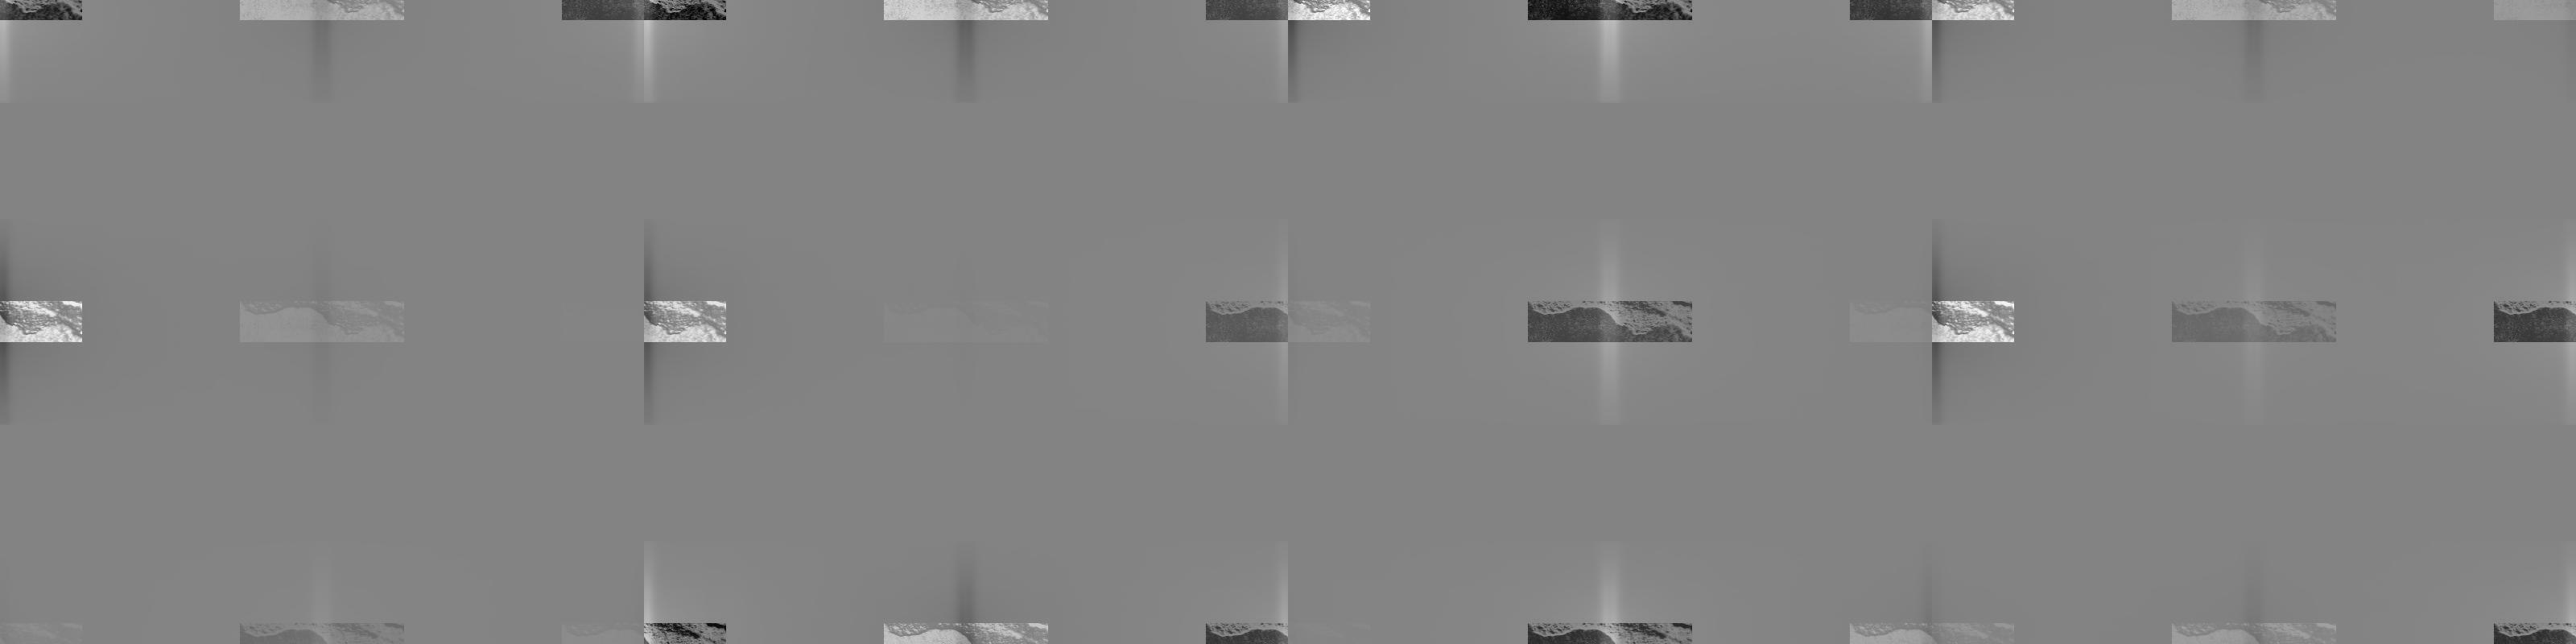
\includegraphics[width=\textwidth,angle=90]{graphics/architecture/act_net_hope}
            }
            \only<20-21> {
                \begin{columns}
                    \column{.5\linewidth}
                    \centering
                    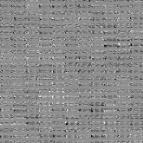
\includegraphics[width=\linewidth]{graphics/architecture/act_net_out}
                    \only<13> {$512\times 512$}
                    \column{.5\linewidth}
                    \centering
                    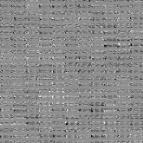
\includegraphics[width=\linewidth]{graphics/architecture/act_net_hope_out}
                    \only<13> {$128\times 128$}
                \end{columns}
            }
            \only<2-3> {
                \begin{itemize}
                    \item \textbf{Convolutional Layer}
                    \item $8/16$ $\left[3\times 3\times 4/16\right]$ filters
                    \item Stride $\left[1\;1\right]$
                    \item Padding ``same''
                    \only<3> {
                        \item \textbf{Max Pooling}
                        \item $\left[4\times 4\times 1\right]$
                        \item Stride $\left[4\;4\right]$
                        \item Padding ``same''
                    }
                \end{itemize}
            }
            \only<4-5> {
                \begin{itemize}
                    \item \textbf{Convolutional Layer}
                    \item $32/64/128$ $\left[3\times 3\times 16/32/64\right]$ filters
                    \item Stride $\left[1\;1\right]$
                    \item Padding ``same''
                    \only<5> {
                        \item \textbf{Max Pooling}
                        \item $\left[2\times 2\times 1\right]$
                        \item Stride $\left[2\;2\right]$
                        \item Padding ``same''
                    }
                \end{itemize}
            }
            \only<6> {
                \begin{itemize}
                    \item \textbf{Fully Connected}
                    \item $16/16/4$ neurons
                \end{itemize}
            }
            \only<7> {
                \begin{itemize}
                    \item \textbf{Softmax}
                    \item $c_i = \frac{e^{o_i}}{\sum_{k = 1}^4 e^{o_k}}$
                \end{itemize}
            }
    \end{columns}
\end{frame}

% \begin{frame}
%     \frametitle{Results}
%     \framesubtitle{Local Column - Equalization}
%     \centering
%     \begin{columns}
%         \column{0.5\textwidth}
%             \onslide <1-> {
%                 \includegraphics[width=\linewidth]{graphics/results/spreader-net-confusion-noneq}
%             }
%         \column{0.5\textwidth}
%             \onslide <2-> {
%                 \includegraphics[width=\linewidth]{graphics/results/spreader-net-confusion}
%             }
%     \end{columns}
% \end{frame}

% \begin{frame}
%     \frametitle{Results}
%     \framesubtitle{Local Column - Spreader vs Crop}
%     \centering
%     \begin{columns}
%         \column{0.5\textwidth}
%             \onslide <1-> {
%                 \includegraphics[width=\linewidth]{graphics/results/spreader-net-confusion}
%             }
%         \column{0.5\textwidth}
%             \onslide <2-> {
%                 \includegraphics[width=\linewidth]{graphics/results/crop-net-confusion}
%             }
%     \end{columns}
% \end{frame}